% Chapter Template

\chapter{Podstawowe czujniki w kwadrokopterach} % Main chapter title

\label{Chapter4} % Change X to a consecutive number; for referencing this chapter elsewhere, use \ref{ChapterX}

\lhead{Chapter 4. \emph{Czujniki w kwadrokopterach}} % Change X to a consecutive number; this is for the header on each page - perhaps a shortened title

%----------------------------------------------------------------------------------------
%	SECTION 1
%----------------------------------------------------------------------------------------
\section{Algorytm -> regulator -> czujnik}

W poprzednim rozdziale opisane były podstawowe algorytmy kontroli i stabilizacji lotu kwadrokopterów. Algorytmy te łączyła jedna podstawowa cecha wspólna - wykorzystanie sprzężenia zwrotnego, w którym informacja o rzeczywistym stanie systemu (prędkości obrotowe lub położenie kątowe) była przekazywana jako jedna z informacji na wejście regulatorów wykorzystanych w algorytmie. Informacja ta pochodzi z odpowiednich czujników: akcelerometrów i żyroskopów. Dzięki niej, kontroler lotu może dokonywac odpowiednich poprawek w sygnałach sterujących silnikami w celu utrzymania zadanych parametrów lotu. Widać zatem że czujniki odgrywają jedną z kluczowych ról w całym procesie stabilizacji i kontroli lotu kwadrokoptera. 

Obecnie na rynku dostępne są rozmaite czujniki zdolne do pomiarów różnych wielkości fizycznych. Do najbardziej popularnych czujników, z których korzysta się przy konstruowaniu modeli latających należą:

\begin{itemize}
	\item \textbf{Akcelerometry - czujniki służące do pomiaru wartości przyspieszeń liniowych}
	\item \textbf{Żyroskopy - czujniki służące do pomiaru wartości prędkości kątowych}
	\item Magnetometry - czujniki służące do pomiaru natężenia pól magnetycznych
	\item Barometry - czujniki służące do pomiaru ciśnienia atmosferycznego
\end{itemize}

Wszystkie te czujniki mogą zostać użyte do określania położenia kwadrokptera w przestrzeni, jednakże jako że dwa z nich (akcelerometry i żyroskopy) stanowią niezbędne minimum, tylko one będą omawiane w dalszej części tego rozdziału.

Po zawężeniu obszaru poszukiwań czujników jedynie do żyroskopów i akcelerometrów, użytkownik nadal pozostaje z bardzo szerokim wachlarzem dostępnych sensorów. Należy zatem dokonać wyboru elementu najbadziej pasującego do wymagań aplikacji na podstawie parametrów takich jak:

\begin{itemize}
	\item Rodzaj wyjścia
		\begin{itemize}
			\item Analogowe
			\item Cyfrowe (np. I\textsuperscript{2}C lub SPI)
		\end{itemize}
	\item Maksymalny zakres pomiarowy
	\item Dokładność pomiarowa
	\item Maksymalna częstotliwość próbkowania
	\item Zakres napięć zasilania
\end{itemize}

Z punktu widzenia potencjalnego użytkownika kluczowymi parametrami dobieranych czujników są interfejsy komunikacyjne (w przypadku interfejsów cyfrowych również rodzaj użytego protokołu) a także maksymalny zakres pomiarowy.

\section{Technologia MEMS}

Rozmaitość typów czujników dostępnych na rynku wiąże się z jeszcze większą rozmaitością dostępnych technologii ich wykonania. Wśród popularnych techologii, można wyróżnić:

\begin{itemize}
	\item Mechaniczne
	\item Optyczne
	\item \textbf{Elektromechaniczne - technologia MEMS}
\end{itemize}

Wiele obecnie wykorzystywanych technologii umożliwia stworzenie bardzo czułych i dokładnych czujników (np. Żyroskopy laserowe należą do jednych z najczulszych i najdokładniejszych żyroskopów). Posiadają one jednak poważne wady z punktu widzenia montażu na modelu kwadrokoptera takie jak zbyt duże rozmiary i zbyt duża masa. 

W ostatnich latach, rozwój technologii MEMS, umożliwił tworzenie czujników, które dzięki swoim niewielkim rozmiarom oraz małej masie stanowią idealne rozwiązanie dla bezzałogowych kontstrukcji latających. 

MEMS (ang. Micro Electro Mechanical Systems) jest terminem określającym technologię wytwarzania miniaturowych systemów elektromechanicznych, których wymiary fizyczne mieszczą się w przedziale od milimetrów do pojedynczych mikrometrów. Dzięki omawianej technologii można wykonywać rozmaite rodzaje urządzeń, od nieskomplikowanych systemów bez żadnych ruchomych elementów po bardzo złożone struktury zawierające dziesiątki ruchomych elementów sterowanych za pomocą zintegrowanych układów elektronicznych. 

\begin{figure}[H]
	\centering
	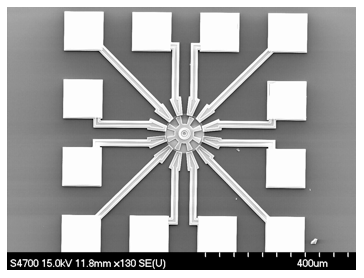
\includegraphics[scale=0.7]{Pictures/microactuator.png}
		%\rule{35em}{0.5pt}
		\caption[Miniaturowy silnik wykonany w technologii MEMS]{Miniaturowy silnik wykonany w technologii MEMS}
	\label{fig:microactuator}
\end{figure}

\begin{figure}[H]
	\centering
	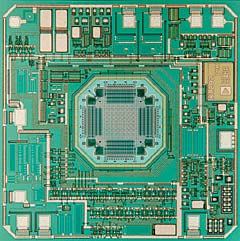
\includegraphics[scale=0.7]{Pictures/3d_accel.jpg}
		%\rule{35em}{0.5pt}
		\caption[Struktura trzyosiowego akcelerometru wraz ze zintegrowanymi układami elektronicznymi]{Struktura trzyosiowego akcelerometru wraz ze zintegrowanymi układami elektronicznymi}
	\label{fig:3d_accelerometer}
\end{figure}

Rysunki ~\ref{fig:microactuator} oraz ~\ref{fig:3d_accelerometer} przedstawiają przykładowe struktury wykonane przy użyciu technologii MEMS. 

Do produkcji struktur MEMS, najczęściej wykorzystuje się krzem, głównie ze względu na jego właściwości fizyczne oraz z uwagi na bardzo dużą dostępność płytek monokryształów tego pierwiastka, stanowiących podłoże produkcyjne. Dzięki temu, struktury MEMS mogą być integrowane z układami elektronicznymi w obrębie pojedynczego układu scalonego. Widać to na przykładzie rysunku ~\ref{fig:3d_accelerometer} prezentującego jedną z możliwych konstrukcji trzyosiowego akcelerometru. Specjalizowane układy elektroniczne mierzą przyspieszenia liniowe działające na centralnie umieszczoną strukturę MEMS. Dzięki takim rozwiązaniom możliwe jest tworzenie miniaturowych elektromechanicznych czujników, które przy zachowaniu przyzwoitych parametrów cechują się bardzo niską ceną.   

\section{Akcelerometr}

Istnieje wiele sposobów na stworzenie akcelerometru. Jedną z nich jest wykorzystanie materiałów piezoelektrycznych i mierzenie wytwarzanych przez nie napięć, proporcjonalnych do wartości przyspieszenia. Czujniki wykonane w tej technologii są jednak zazwyczaj stosunkowo duże i nie nadawałyby się do wykorzystania w konstrukcjach latających. Akcelerometry MEMS wykorzystują zmianę pojemności kondensatorów płaskich, będących elementem ich elektromechanicznej struktury.

Metoda pomiaru pojemności kondensatorów niesie ze sobą wiele zalet. Proces produkcji takich struktur jest bardzo prosty i nie wymaga dużych nakładów pracy. Dodatkowo pojemność kondensatorów złożonych z równoległych powierzchni wyrażana wzorem:   

\begin{equation}
C = \epsilon_0\epsilon_r\frac{S}{d}
\end{equation}

gdzie $\epsilon_0$ oznacza względną przenikalność elektryczną próżni, $\epsilon_r$ wzdlęgną przenikalność elektryczną izolatora między okładkami kondensatora, $S$ powierzchnię okładek a $d$ odległość między okładkami, nie zależy od temperatury, dzięki czemu czujniki zbudowane w oparciu o pomiar pojemności cechują się dużą dokładnością. Z powyższego wzoru widać, że kondensator płaski może również pełnić rolę na przykład czujnika wilgotności - wartość $\epsilon_r$ będzie zmieniać się wraz ze zmianą zawartości pary wodnej w powietrzu. Jednak w przypadku akcelerometrów interesować nas będzie zmiana pojemności wynikająca ze zmiany odległości między okładkami proporcjonalnej do przyspieszeń linowych.

\begin{figure}[H]
	\centering
	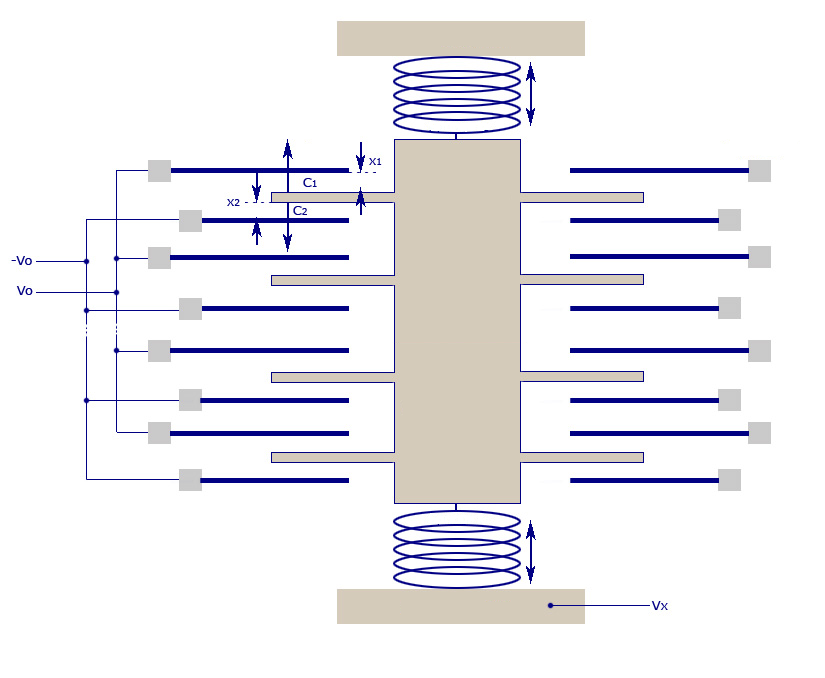
\includegraphics[scale=0.4]{Pictures/MEMS-Accelerometer_struct.png}
		%\rule{35em}{0.5pt}
		\caption[Zasada działania akcelerometru MEMS]{Zasada działania akcelerometru MEMS}
	\label{fig:MEMS-Accelerometer_struct}
\end{figure}

Rysunek ~\ref{fig:MEMS-Accelerometer_struct} przedstawia budowę i zasadę działania akcelerometru MEMS. Składa się on z ruchomej masy odniesienia, zamocowanej za pomocą sprężyn do ramy pokrywającej się z układem odniesienia urządzenia. Masa odniesienia posiada okładki, które wraz z nieruchomymi okładkami zewnętrznej ramy tworzą kondensatory płaskie. Przesunięcie liniowe masy odniesienia, proporcjonalne do przyspieszenia działającego na układ może być mierzone za pomocą różnicy pojemności $C1$ i $C2$ co opisują poniższe wzory:

\begin{equation}
\begin{aligned}
C1 &= \epsilon_0\epsilon_r\frac{S}{d + x} &= C_0 - \Delta{C} \\
C2 &= \epsilon_0\epsilon_r\frac{S}{d - x} &= C_0 + \Delta{C}
\end{aligned}
\label{C_to_delta}
\end{equation} 

W przypadku braku przyspieszenia działającego na układ, różnica pojemności wynosi $0$ ponieważ $x_1 = x_2$. W przypadku działania przyspieszenia, różnicę pojemności wynikającą z faktu że $x_1 \neq x_2$ można wyrazić wzorem:

\begin{equation}
	C_2 - C_1 = 2\Delta{C} = 2\epsilon_0\epsilon_rS\frac{x}{d^2 - x^2}
\end{equation}

Chcąc wyznaczyć przesunięcie x, należy rozwiązać równanie kwadratowe:

\begin{equation}
	\Delta{C}x^2 + \epsilon_0\epsilon_rSx - \Delta{C}d^2 = 0
\end{equation}

Równanie to można jednak uprościć, jako że dla niewielkich przesunięć człon $\Delta{C}x^2$ można pominąć. Zatem równanie kwadratowe upraszcza się do postaci:

\begin{equation}
	x \approx \frac{d^2}{\epsilon_0\epsilon_r}\Delta{C} = d\frac{\Delta{C}}{C_0}
	\label{x_to_c}
\end{equation}

Jak widać na rysunku ~\ref{fig:MEMS-Accelerometer_struct} pojemności $C_1$ oraz $C_2$ składają się z wielu ( z reguły około kilkudziesięciu)  kondensatorów płaskich połączonych równolegle. Gdyby nie zastosować takiej konstrukjci, pojemność wytwarzana przez pojedynczą parę okładek byłaby tak mała, że powodowałoby to znaczne trudności podczas jej pomiaru. 

\begin{figure}[H]
	\centering
	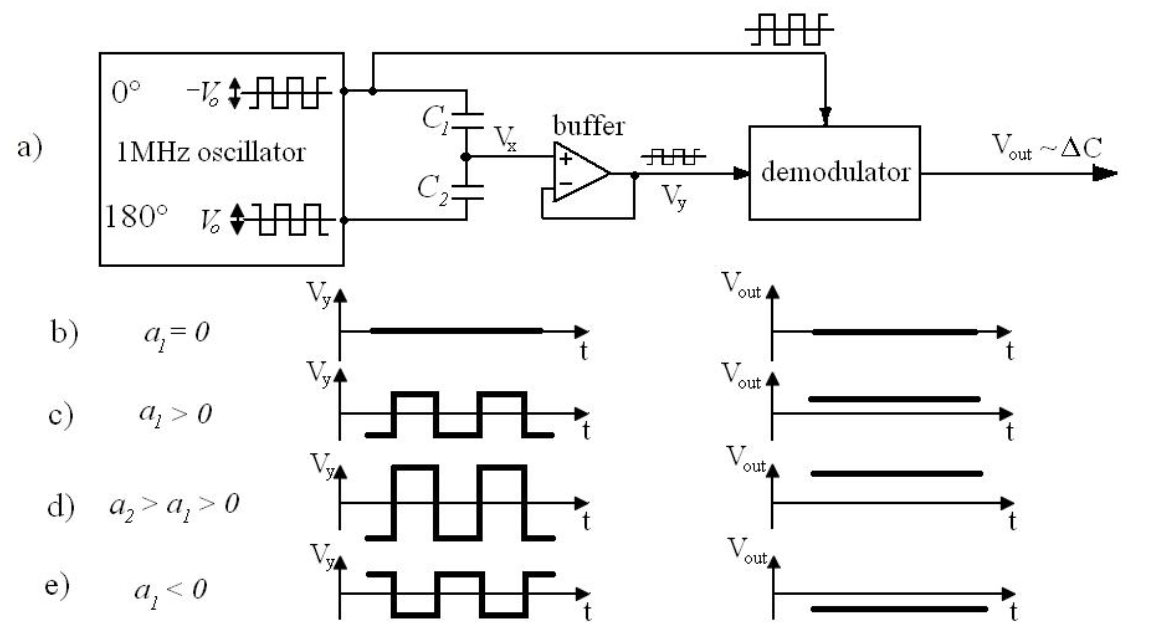
\includegraphics[scale=0.4]{Pictures/MEMS_accel_demod.png}
		%\rule{35em}{0.5pt}
		\caption[Układ elektroniczny do pomiaru różnicy pojemności kondensatorów]{a) Układ elektroniczny mierzący przyspieszenia na podstawie zmiany pojemności kondensatorów b,c,d,e) przebiegi sygnału na wyjściu wtórnika napięciowego oraz wartości napięć wyjściowych układu, dla różnych wartości przyspieszeń }
	\label{fig:MEMS_accel_demod}
\end{figure}

Na rysunku ~\ref{fig:MEMS_accel_demod} przedstawiono najprostszą postać układu służącego do pomiaru przyspieszeń liniowych na podstawie zmiany pojemności kondensatorów. Składa się on z oscylatora, generującego dwa przebiegi prostokątne częstotliwości 1MHz oraz amplitudzie $V_0$, przesunięte względem siebie w fazie o $180\,^{\circ}$. Oba te przebiegi podłączone do pary kondensatorów $C_1$ i $C_2$ generują sygnał $V_x$, który jest napięciem masy odniesienia. Można to zapisać za pomocą następujących wzorów:

\begin{equation}
	(V_x + V_0)C_1 + (V_x + C_0)C_2 = 0
\end{equation}  

Korzystając z równań ~\ref{C_to_delta} oraz ~\ref{x_to_c}, powyższą zależność można przedstawić w następującej postaci:

\begin{equation}
V_x = V_0\frac{C_2 - C_1}{C_2 + C_1} = \frac{x}{d}V_0
\label{vx_to_x}
\end{equation}

zatem $V_x$ jest również przebiegiem prostokątnym, o amplitudzie proporcjonalnej do liniowego przesunięcia masy odniesienia. Sygnał ten jest jednak bardzo słaby, dlatego też trafia dalej do układu, który go wzmacnia (w przypadku układu z rysunku ~\ref{fig:MEMS_accel_demod} jest to zwykły wtórnik napięciowy) a następnie trafia do demodulatora wraz z jednym z sygnałów oscylatora. Na wyjściu demodulatora można już zaobserwować sygnał, którego wartość jest proporcjonalna do przyspieszenia. Ostatnim z czynników, który musi być brany pod uwagę podczas wyznaczania przyspieszenia za pomocą tego typu czujnika są sprężyny, którymi masa odniesienia zamocowana jest do zewnętrznej ramy. Na podstawie prawa Hooke'a wiadomo, że zmiana długości sprężyny $x$ jest proporcjonalna do zewnętrznej siły $F_s$ która na nią działa. Łącząc prawo Hooke'a z drugą zasadą dynamiki Newtona, można zapisać następujące równanie, opisujące zależność między przemieszczeniem $x$ masy odniesienia akcelerometru a przyspieszeniem, które na nią działa:

\begin{equation}
	a = \frac{k_s}{m}x
\end{equation}  

gdzie $a$ to wartość przyspieszenia, $k_s$ to współczynnik sprężystości sprężyn mocujących masę odniesienia ro zewnętrznej ramy, $m$ to masa masy odniesienia a $x$ to wartość przemieszczenia. Wykorzystując równanie ~\ref{vx_to_x} można zapisać ostateczną postać wzoru, pozwalającą wyznaczyć wartość przyspieszenia w funkcji napięcia wyjściowego układu przedstawionego na rysunku ~\ref{fig:MEMS_accel_demod}

\begin{equation}
	a = \frac{k{_s}d}{mV_0}V_x
\end{equation}

\section{Żyrosop}

Żyrosop służy pomiaru prędkości obrotowej. Jako że stabilizacja lotu kwadrokoptera w najprostrzej postaci polega na utrzymaniu stałej prędkości kątowej wokół każdej z trzech osi, żyroskop jest kluczowym czujnikiem, w jaki wyposaża się kwadrokopter. 

Żyroskopy MEMS należą do grupy żryroskopów z wibrującą strukturą, mierzących prędkość kątową dzięki sile Coriolisa. W wyniku jej działania ciało, w żyroskopach jest to z reguły odpowiednio przygotowana miniaturowa płytka krzemu, wprawione w wibracje w określonej płaszczyźnie będzie dążyć do utrzymania wibracji w tej płaszczyźnie mimo obrotu ramy, do której ciało to jest przymocowane. Chcąc uświadomić sobie jak innowacyjna jest to konstrukcja warto najpierw omówić dwa najbardziej popularne typy żyroskopów - żyroskop mechaniczny oraz żyroskop laserowy.

\begin{figure}[H]
	\centering
	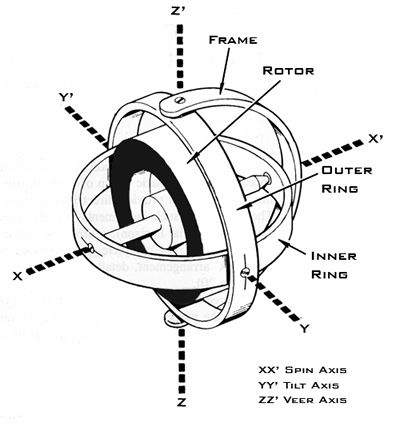
\includegraphics[width=0.6\textwidth]{Pictures/Gyroscope_Theory.jpg}
	%\rule{35em}{0.5pt}
	\caption[Przykład żyroskopu mechanicznego]{Przykład żyroskopu mechanicznego}
	\label{fig:Gyroscope_Theory}
\end{figure}

Rysunek ~\ref{fig:Gyroscope_Theory} przedstawia przykładową budowę żyroskopu mechanicznego. Głównym elementem jest dysk wirujący z dużą prędkością, który utrzymuje stałe położenie kątowe. Osadzony jest w ramie, zazwyczaj w formie trzech pierścieni, umożliwiającej jego swobodny obrót wokół trzech osi. Dzięki temu wirująca masa może zachować swoje stałe położenie kątowe względem Ziemi niezależnie od obrotu urządzenia, w którym zamontowano żyroskop. Warto zauważyć, że poprzez umieszczenie enkoderów na styku pierścieni ramy, za pomocą tego typu żyroskopu można zmierzyć nie tylko prędkość kątową ale również ukreślić położenie kątowe żyroskopu, co z punktu widzenia algorytmów kontroli jest bardzo cenną cechą tych czujników. 

Zdecydowaną wadą żyroskopów mechanicznych jest ich duża masa, oraz występowanie w ich wnętrzu wirujących elementów. W celu eliminacji tych wad, opracowano nowe rodzaje żyroskopów takie jak żyroskopy laserowe, działające w oparciu o efekt Sagnaca.

\begin{figure}[H]
	\centering
	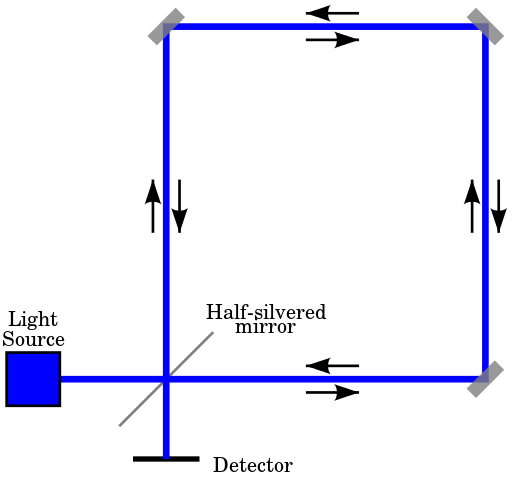
\includegraphics[scale=0.4]{Pictures/Sagnac_interferometer.png}
        %\rule{35em}{0.5pt}
        \caption[Zasada działania żyroskopów laserowych]{Zasada działania żyroskopów laserowych}
        \label{fig:300px-SagnacPhase}
\end{figure}

Rysunek ~\ref{fig:300px-SagnacPhase} przedstawia zasasdę działania żyroskopu laserowego, zwanego również interferometrem Sagnaca. Promień światła rostaje rodzielony na dwie wiązki, które następnie przebywają tę sasmą drogę w przeciwnych kierunkach. W wyniku ruchu obrotowego urządzenia, powstaje subtelna różnica w fazie między dwoma wiązkami, którą następnie można zauważyć w postaci prążków interfencyjnych. Żyroskopy wykorzystujące efekt Sagnaca należą do grupy bardzo precyzyjnych czujników, częściowo ze względu na swoją niewrażliwość na przyspieszenia liniowe oraz wibracje. Z tego względu stosuje się je głównie z aplikacjach lotniczych (samoloty pasażerskie), militarnych (zdalnie naprowadzane rakiety), oraz astronautycznych (międzynarodowa stacja kosmiczna). 

\begin{figure}[H]
	\centering
	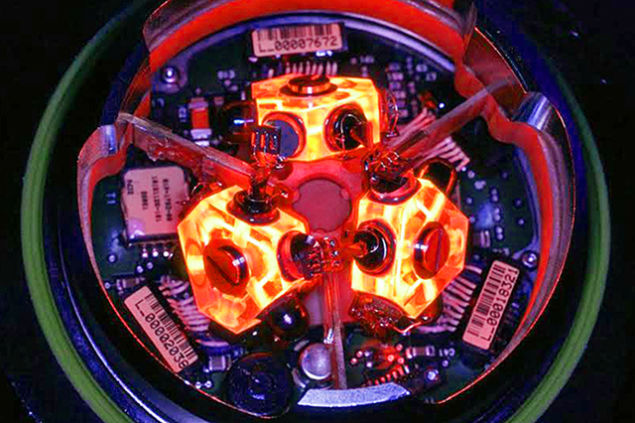
\includegraphics[scale=0.4]{Pictures/3d_laser_ring_gyro.jpg}
        %\rule{35em}{0.5pt}
        \caption[Trzyosiowy żyroskop laserowy]{Trzyosiowy żyroskop laserowy}
        \label{fig:3d_laser_ring_gyro}
\end{figure}

Rysunek ~\ref{fig:3d_laser_ring_gyro} przedstawia przykładową konstrukcję trzyosiowego żyroskopy laserowego, używanego w samolotach wojskowych oraz zdalnie naprowadzanych rakietach. 

Jak już wcześniej było wspomniane żyroskopy MEMS, korzystają z zupełnie innych zasad fizycznych niż żyroskopy mechaniczne i laserowe. Zasada ich działania zostanie wytłumaczona na przykładzie trzyosiowego żyroskopu, wykorzystującego odpowiednio ukształtowaną płytkę krzemu do pomiaru prędkości kątowych wokół wszystkich trzech osi jednocześnie.

\begin{figure}[H]
	\centering
	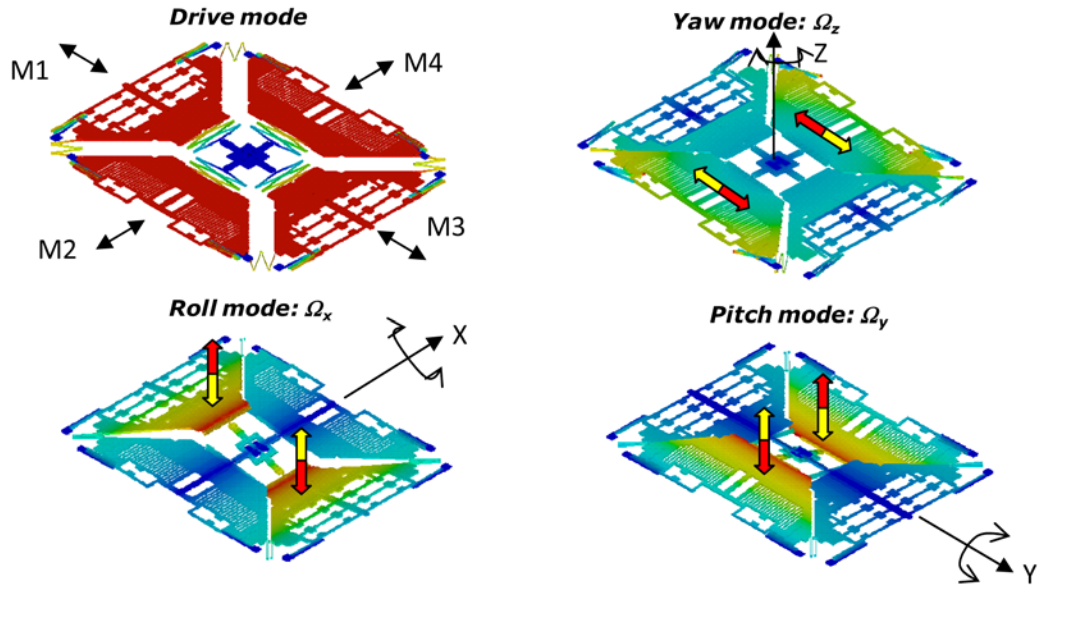
\includegraphics[scale=0.4]{Pictures/3d_gyro.png}
        \caption[Trzyosiowy żyroskop MEMS]{Trzyosiowy żyroskop MEMS}
        \label{fig:3d_gyro}
\end{figure}

W żyroskopie, którego struktura pokazana jest na rysunku ~\ref{fig:3d_gyro} mamy do czynienia z czterema masami $M1$, $M2$, $M3$, $M4$ wibrującymi jednocześnie w płaszczyśnie poziomej. Dzięki takiej strukturze można wykryć prędkości kątowe wokół wszystkich trzech osi. Przy obrocie struktury wokół osi $X$ masy $M1$ oraz $M3$ w wyniku zadziałania siły Coriolisa odchylą się w przeciwne strony wzdłuż osi prostopadłej do płaszczyzny drgań. Odchylenie to może zostać zmierzone za pomocą za pomocą zmiany pojemności kondensatorów płaskich, zawartych w strukturze żyroskopu (kondensatory te będą działały na tej samej zasadzie co kondensatory używane w akcelerometrach MEMS) . Dzięki temu można wyznaczyć wartość prędkości obrotowej wokół osi $X$. Dla obrotu wokół osi $Y$ zachowanie struktury będzie wyglądać analogicznie, z tą różnicą że wychyleniu ulegną masy $M2$ i $M4$. Dla obrotu wokół osi $Z$, dla struktury pokazanej na rysunku masy $M2$ i $M4$ nadal będą drgać w dotychczasowej płaszczyźnie, jednak w wyniku działania siły Coriolisa zaczną drgać w przeciwne strony, co zostało pokazane za pomocą żółtych i czerwonych strzałek.


%----------------------------------------------------------------------------------------
%	SECTION 2
%----------------------------------------------------------------------------------------

\section{Inercyjny zespół pomiarowy - IMU}

Inercyjny zespół pomiarowy jest to zbiór czujników, umożliwiający określenie orientacji statku powietrznego w przestrzeni. Wykorzystuje on najczęściej połączone pomiary z akcelerometrów i żyroskopów, czasem również magnetometrów. Obecnie rozwój technologii MEMS umożliwił tworzenie inercyjnych zespołów pomiarowych zawartych wewnątrz jednego układu scalonego. Przykładem takiego zespołu może być układ MPU-6050, którego struktura przedstawiona jest na poniższym rysunku

\begin{figure}[H]
	\centering
	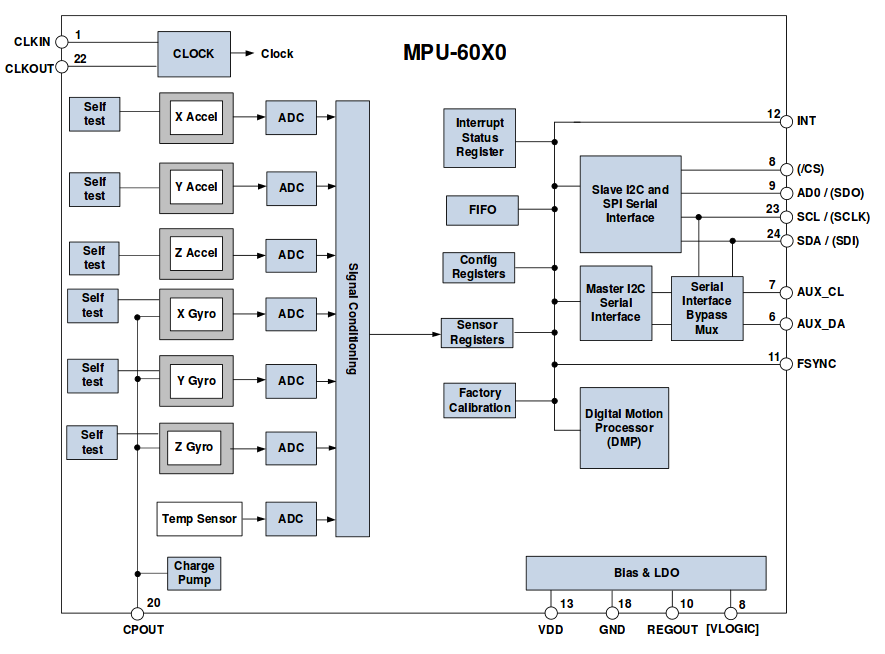
\includegraphics[scale=0.5]{Pictures/IMU.png}
        \caption[Struktura inercjalnego zespołu pomiarowego]{Struktura inercjalnego zespołu pomiarowego MPU-6050}
        \label{fig:IMU}
\end{figure}

Jak widać składa się on z trzyosiowego akcelerometru oraz trzyosiowego żyroskopu oraz wszelkich niezbędnych układów elektronicznych, dzięki którym możliwe jest odczytywanie wartości przyspieszeń linoiowych oraz prędkości kątowych. Układ MPU-6050 został wybrany jako przykład nie bez powodu - zawiera on blok o nazwie DMP (ang. Digital Motrion Procesor) który jest zdolny do automatycznego określania orientacji czujnika w przestrzeni na podstawie pomiarów z żyroskopu i akcelerometru. Jest to unikatowa cecha, dzięki której kontroler lotu wykorzystujący ten czujnik jest zwolniony z konieczności samodzielnego określania  położenia statku powietrznego w przestrzeni. 
